\section{Разработка мобильного модуля.}
\subsection{Разработка структурной схемы.}

Существует несколько вариантов построения оконечного модуля:
\begin{enumerate}
	\item На основе микроконтроллера общего назначения и специализированного приемопередатчика  Semtech из серии SX12**.
	\item На основе готовых микросборок.
	\item На основе специализированных микроконтроллеров.
\end{enumerate}

\justifying В данной работе применяется второй вариант ввиду его простоты. В качестве центрального устройства будет использоваться чип AcSiP S76S. Данный чип представляет из себя микросборку из энергоэффективного МК \linebreak STM32L073xZ, приемопередатчика SX1276 и необходимой периферии. Упрощенная структурная схема МСБ, предоставляемая производителем показана на Рисунке~\ref{fig:S76S-struct}.

\begin{figure}[H]
	\centering
	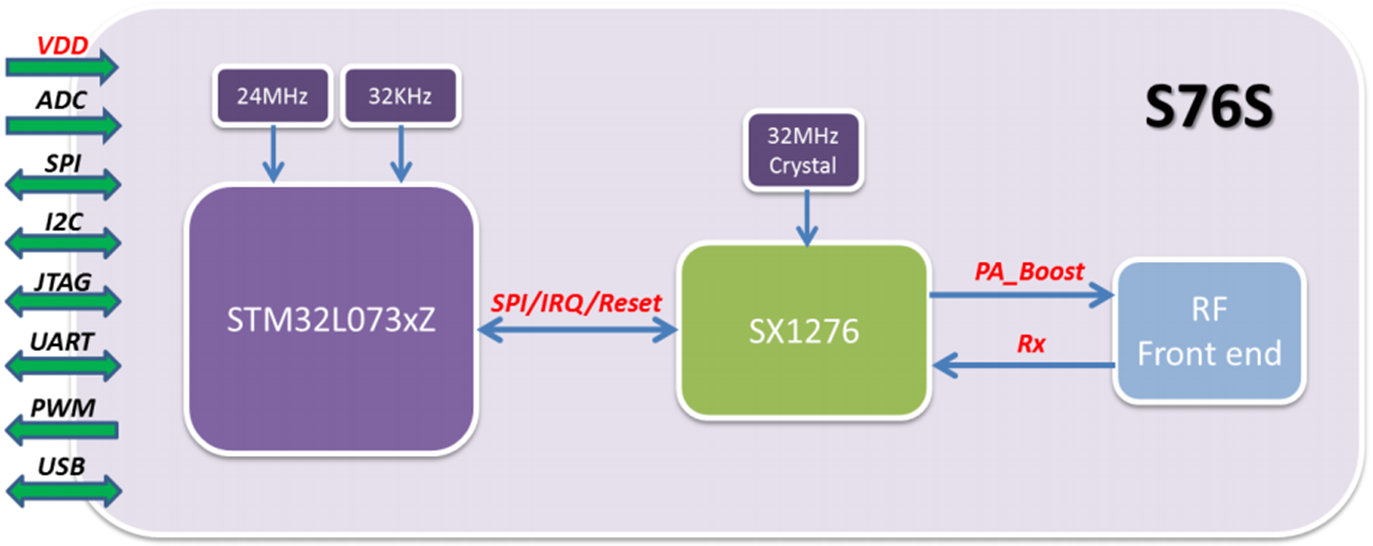
\includegraphics[width=\textwidth,keepaspectratio]{S76S-struct.png}
	\caption{базовая структурная схема AcSiP S76S.}%
	\label{fig:S76S-struct}
\end{figure}

Структурная схема разрабатываемого мобильного модуля показана на Рисунке~\ref{fig:MM-StructSch}

\begin{figure}[H]
	\centering
	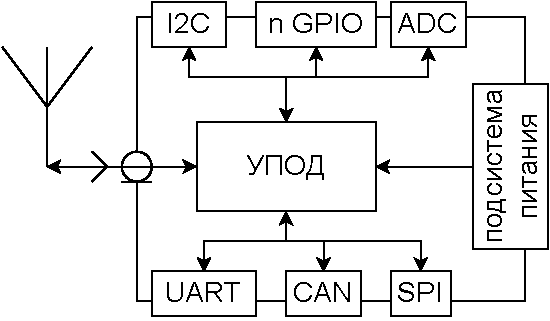
\includegraphics[width=0.8\textwidth,keepaspectratio]{MM-StructSch.pdf}
	\caption{Структурная схема разрабатываемого устройства.\\ УПОД – устройство приёмопередачи и обработки данных.}%
	\label{fig:MM-StructSch}
\end{figure}

\subsection{Разработка подсистемы питания.}

Единственным потребителем электрической энергии на плате является чип S76S, для обеспечения его работы требуется напряжение от 2,4 до 3,6 В. Для обеспечения работы от аккумуляторной батареи с возможностью её зарядки требуется контроллер заряда батареи и стабилизатор напряжения. 

\begin{figure}[H]
	\centering
	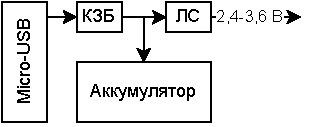
\includegraphics[width=0.7\textwidth,keepaspectratio]{MM-PowerSch.pdf}
	\caption{Структурная схема подсистемы питания МОУ}
	\label{fig:MM-PowerSch}
\end{figure}

\begin{itemize}
	\item На роль линейного стабилизатора выберем описанный ранее LT1965EDD.
	\item Контроллером заряда батареи будет MCP73831T-2ACI/OT с выходным напряжением из ряда 4,2, 4,35, 4,40, 4,50 В и регулируемым выходным током от 15 до 500 мА
	\begin{figure}[H]
		\centering
		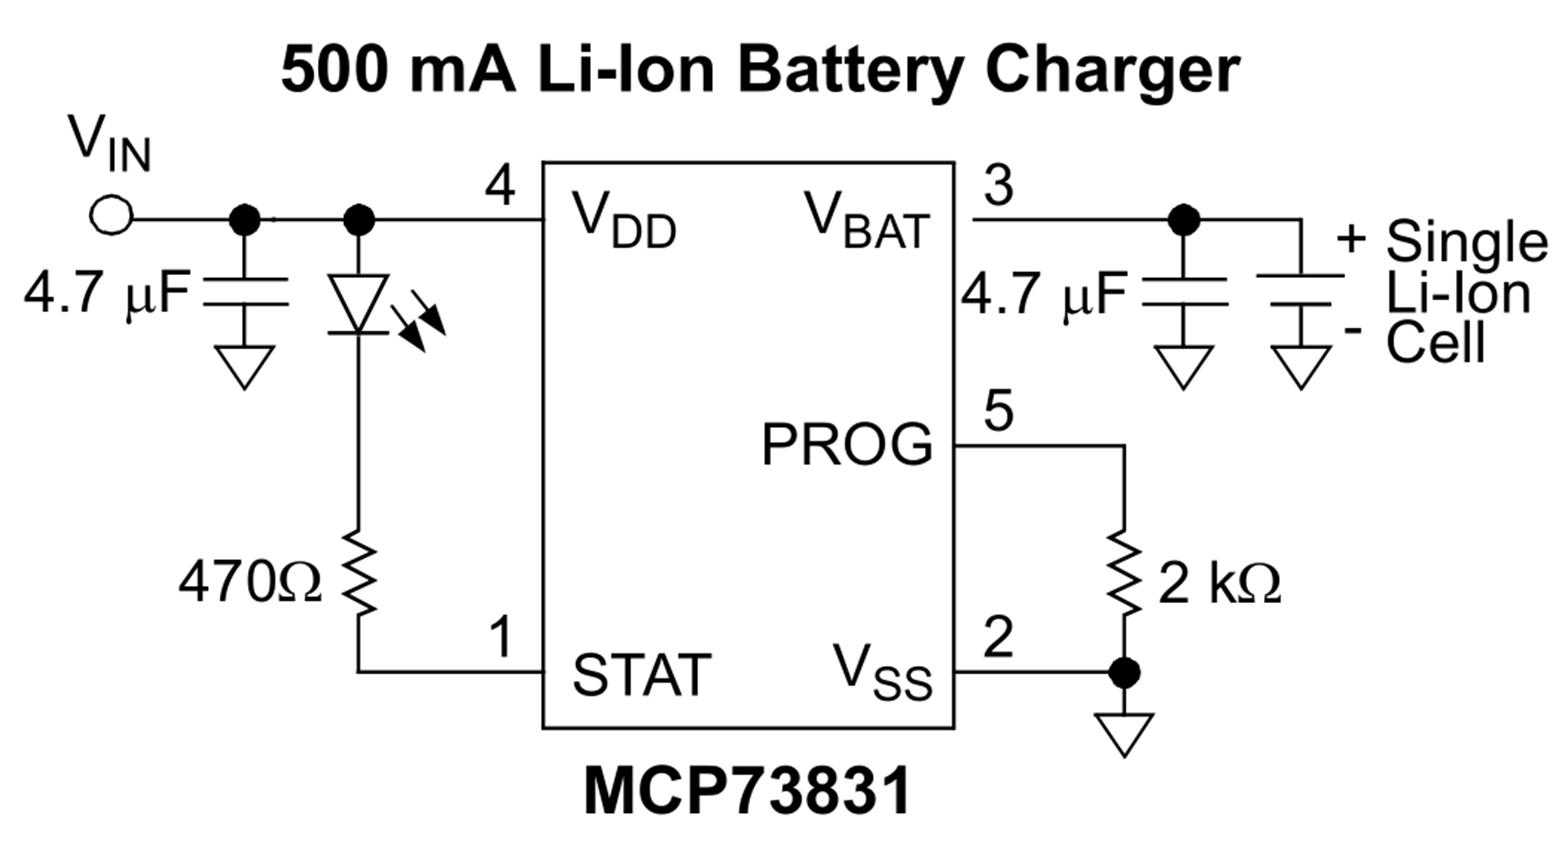
\includegraphics[width=0.8\textwidth,keepaspectratio]{charge-controller.png}
		\caption{стандартная схема включения КЗБУ}
		\label{fig:charge-controller}
	\end{figure}
\end{itemize}

Выбранные компоненты были добавлены в составленную ранее библиотеку.

\subsection{Составление электрической схемы.}

Основываясь на предполагаемых сценариях применения итогового устройства и ориентируясь на рекомендации производителей была составлена электрическая принципиальная схема устройства. Полная документация на устройство будет находиться в репозитории проекта в соответствующем разделе. Более подробно про экспорт документации будет рассказано в главе \ref{sect:project-docs}.

\subsection{Проектирование топологии.}

На основании схемы электрической принципиальной, с использованием составленных ранее библиотек и с учетом возможностей современных производителей печатных плат были спроектированы два варианта топологии печатной платы устройства. Они показаны на рисунках \ref{fig:mb-topology} и \ref{fig:ms-topology}. Первый вариант более удобен для разработки, а также предполагает возможность установки аккумулятора большего объёма. Второй вариант более компактный и предоставляет пользователю выбор типа аккумулятора - со штырьковым разъёмом либо формата АА.

\begin{figure}[H]
	\centering
	\begin{subfigure}[c]{0.49\textwidth}
		\centering
		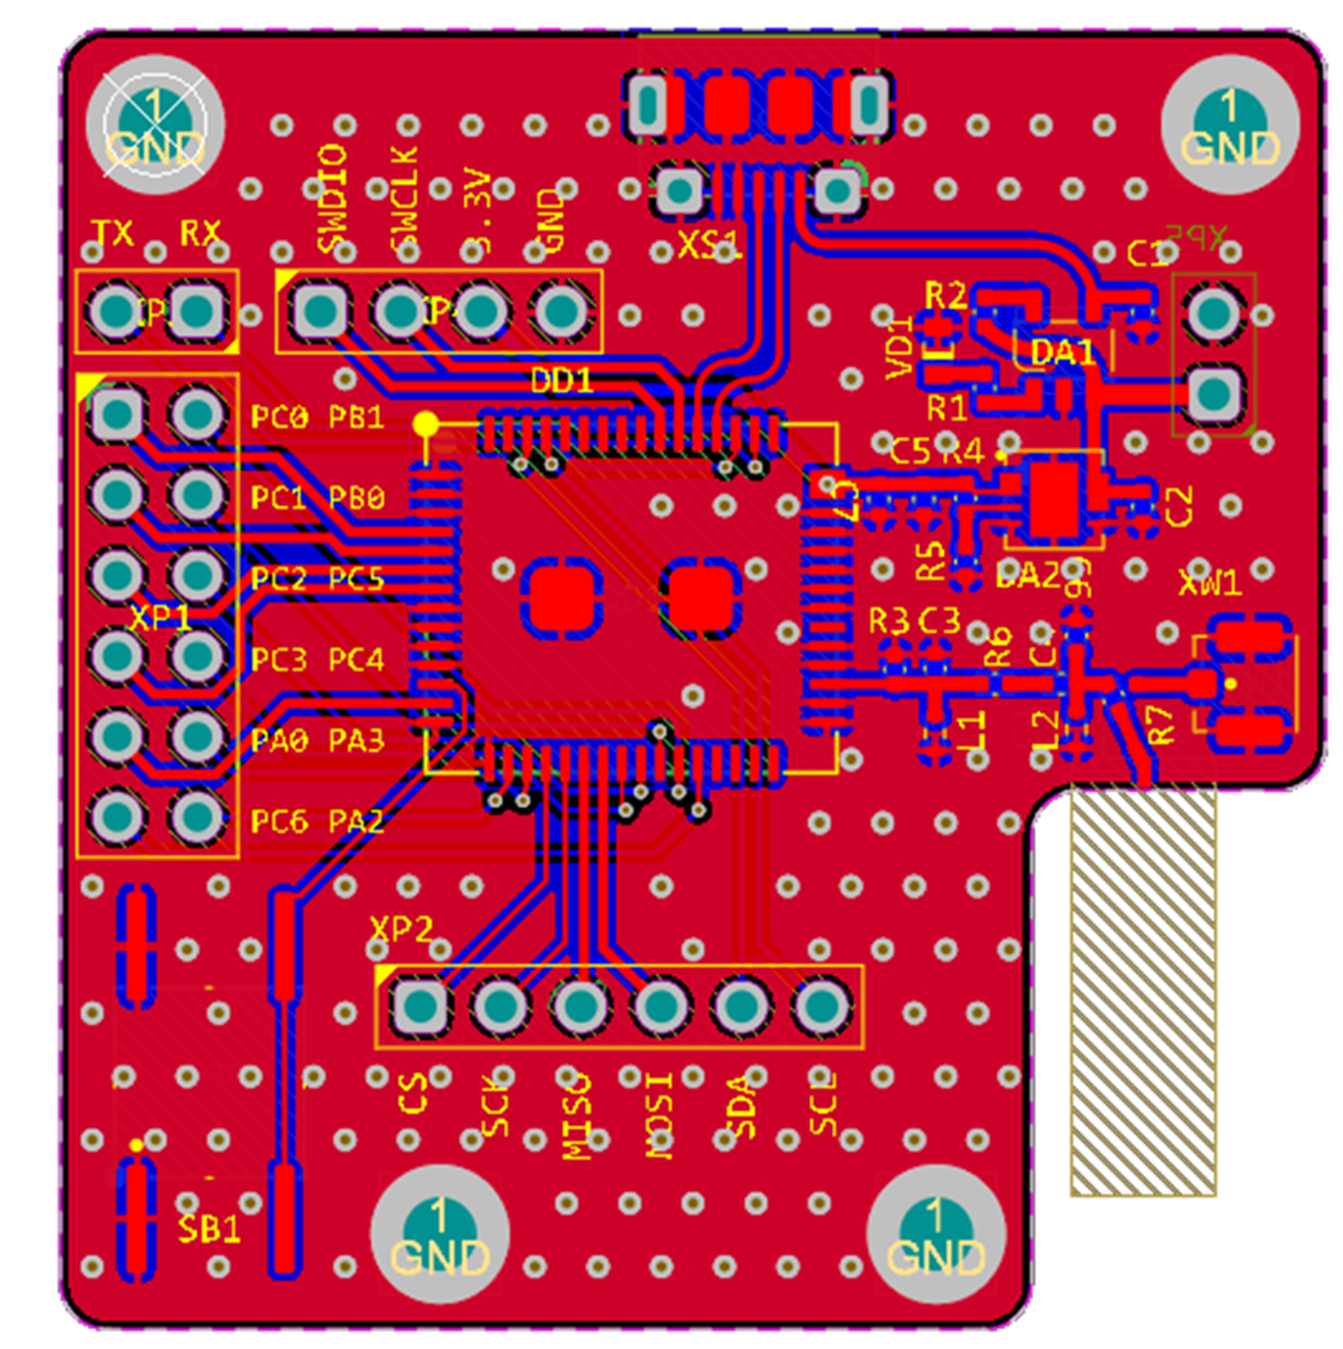
\includegraphics[height=15em]{mb-topology.png}
		\caption{}%
		\label{fig:mb-topology}
	\end{subfigure}
	\hfill
	\begin{subfigure}[c]{0.49\textwidth}
		\centering
		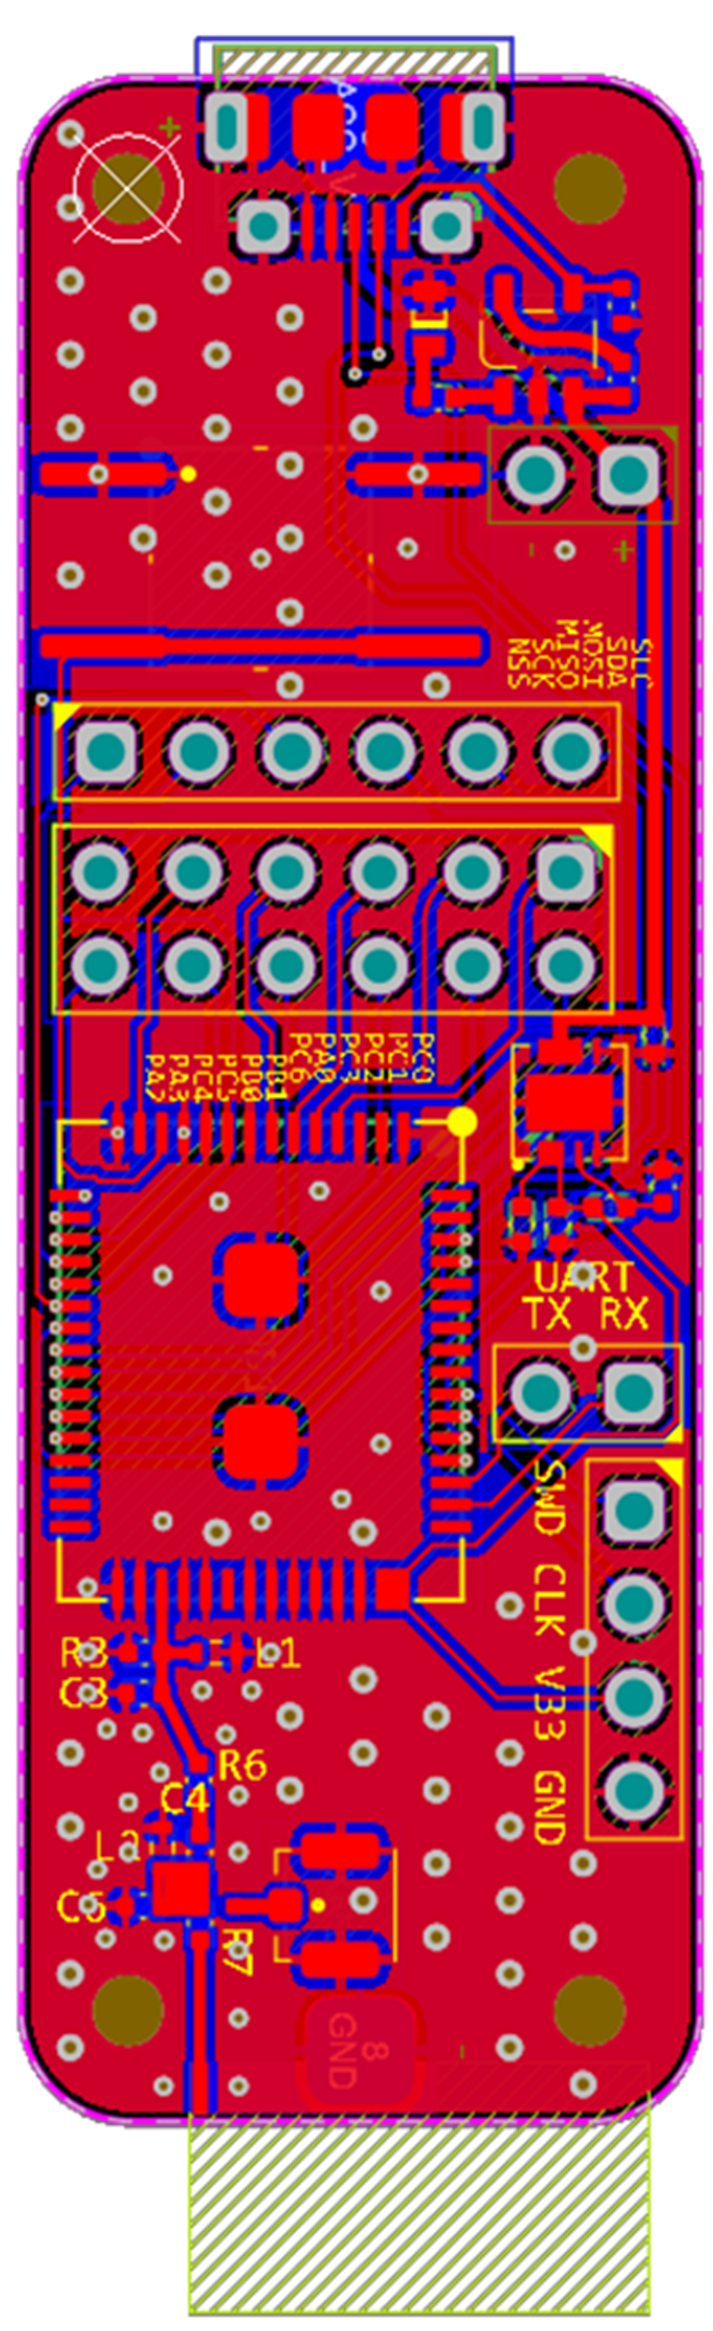
\includegraphics[height=15em]{ms-topology.png}
		\caption{}%
		\label{fig:ms-topology}
	\end{subfigure}
	\caption{%
		Два варианта исполнения платы ММ
	}%
	\label{fig:mm-topology}
\end{figure}

Первый вариант имеет размеры (ШхД) 4х4 см, а второй – 1,2х5,6 см. Заштрихованный блок представляет границы модели предполагаемой антенны. Также предусмотрена возможность подключения антенн к разъёму U.FL и установки чип-антенн.

\begin{figure}[H]
	\centering
	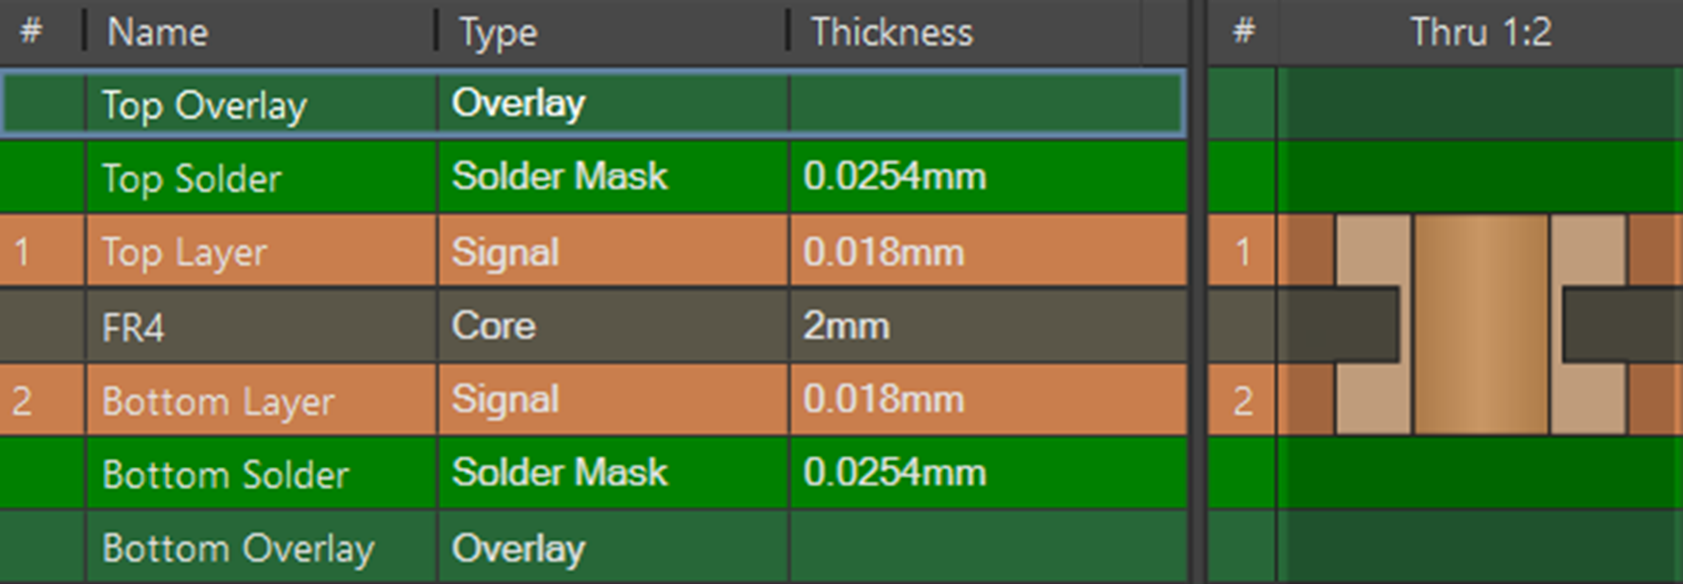
\includegraphics[width=0.7\textwidth,keepaspectratio]{mm-stackup.png}
	\caption{Cтек печатной платы МОУ}
	\label{fig:mm-stackup}
\end{figure}

\begin{figure}[H]
	\centering
	\begin{subfigure}[c]{0.3\textwidth}
		\centering
		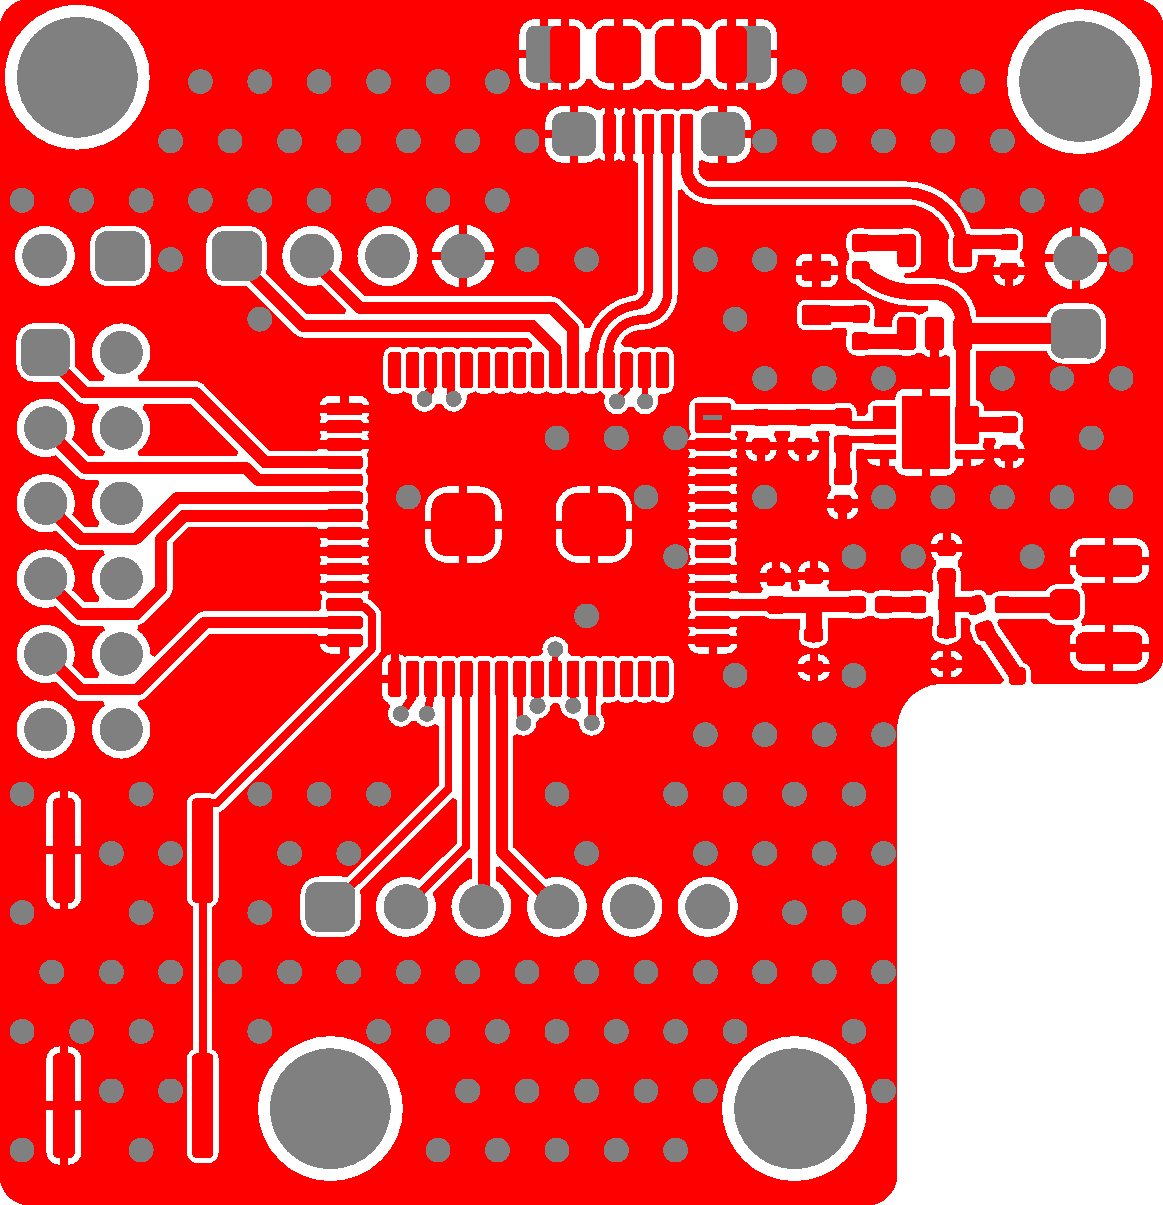
\includegraphics[width=\textwidth, keepaspectratio]{MB-Top Layer.pdf}
		\caption{}%
		\label{fig:MB-TopLayer}
	\end{subfigure}
	\hfil
	\begin{subfigure}[c]{0.3\textwidth}
		\centering
		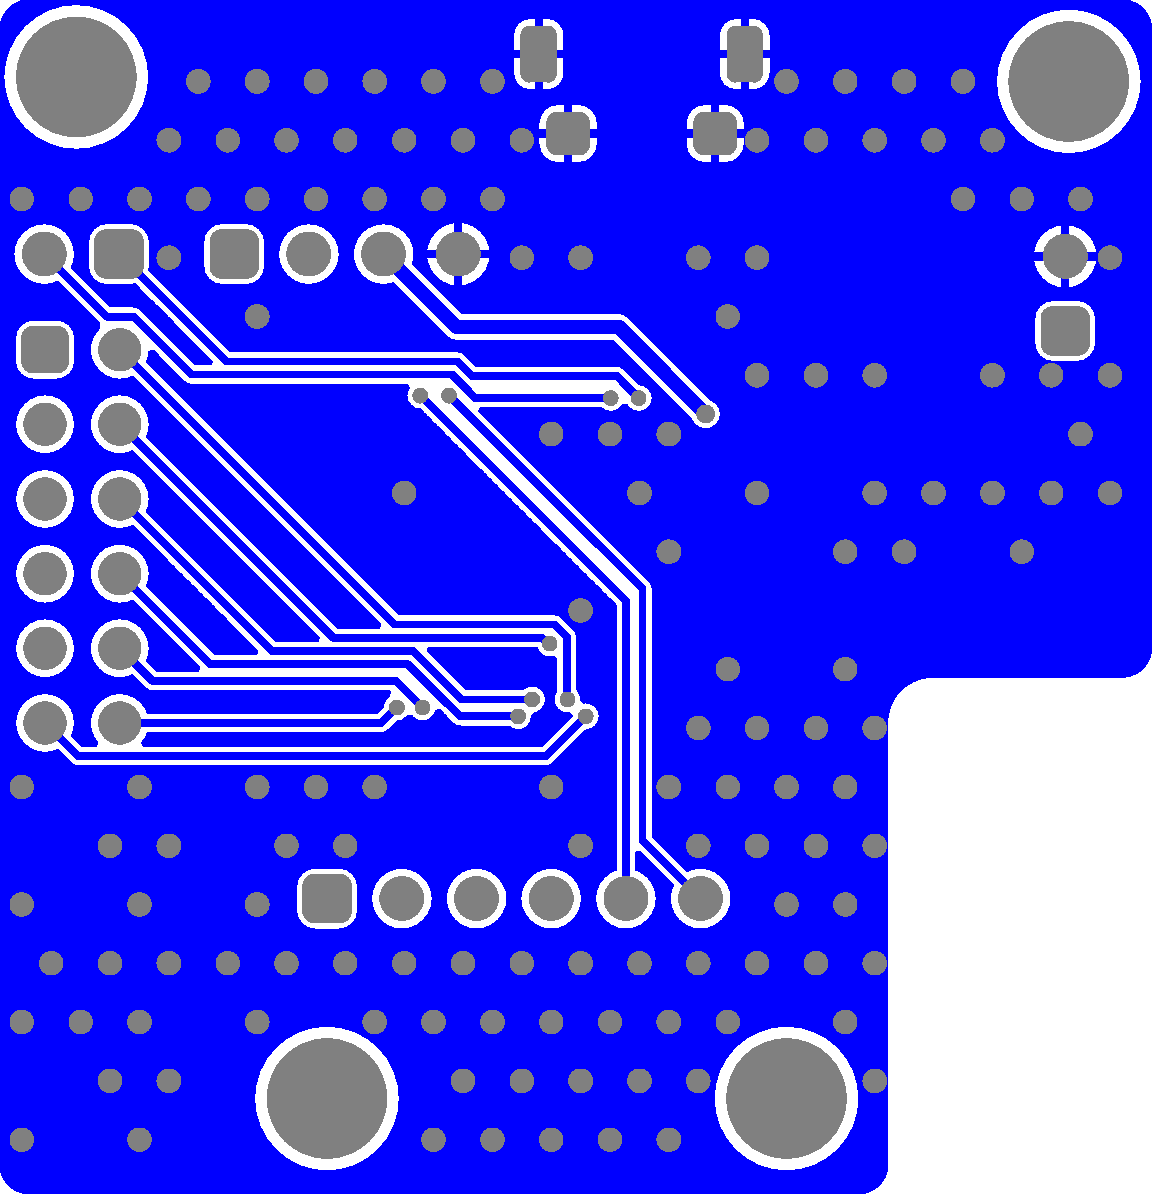
\includegraphics[width=\textwidth, keepaspectratio]{MB-Bottom Layer.pdf}
		\caption{}%
		\label{fig:MB-BottomLayer}
	\end{subfigure}
	\hfil
	\begin{subfigure}[c]{0.3\textwidth}
		\centering
		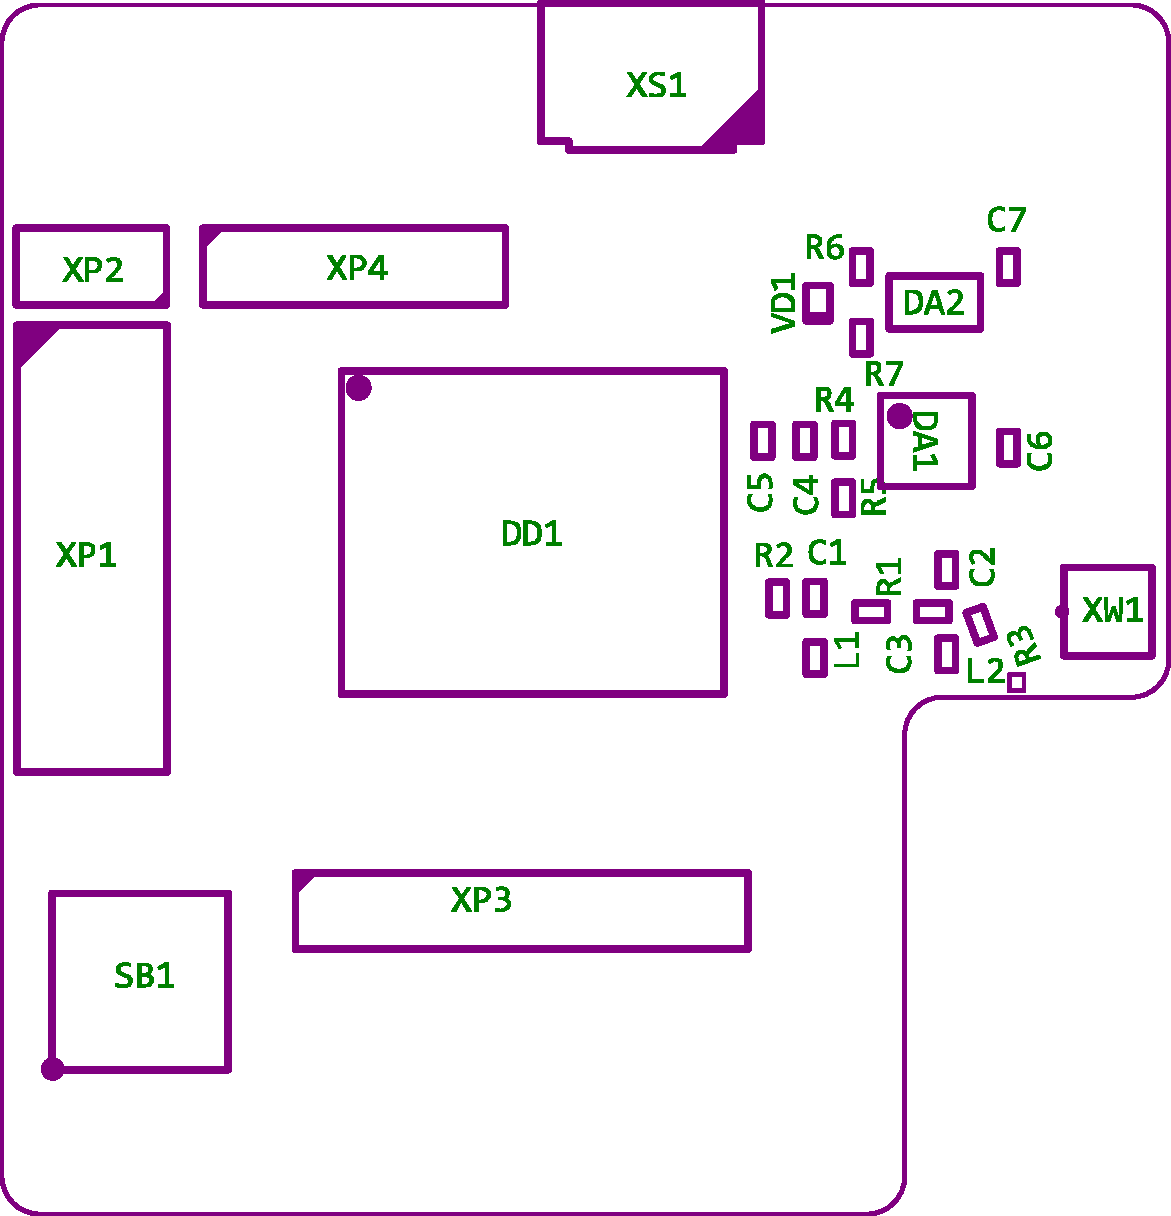
\includegraphics[width=\textwidth, keepaspectratio]{MB-Assembly Drawing.pdf}
		\caption{}%
		\label{fig:MB-AssemblyDrawing}
	\end{subfigure}
	\caption{Первый вариант исполнения. Схемы металлизации (а) верхнего и (б) нижнего слоя. (в) сборочный чертёж верхнего слоя.}
	\label{fig:mb-layers}
\end{figure}

\begin{figure}[H]
	\centering
	\begin{subfigure}[c]{0.325\textwidth}
		\centering
		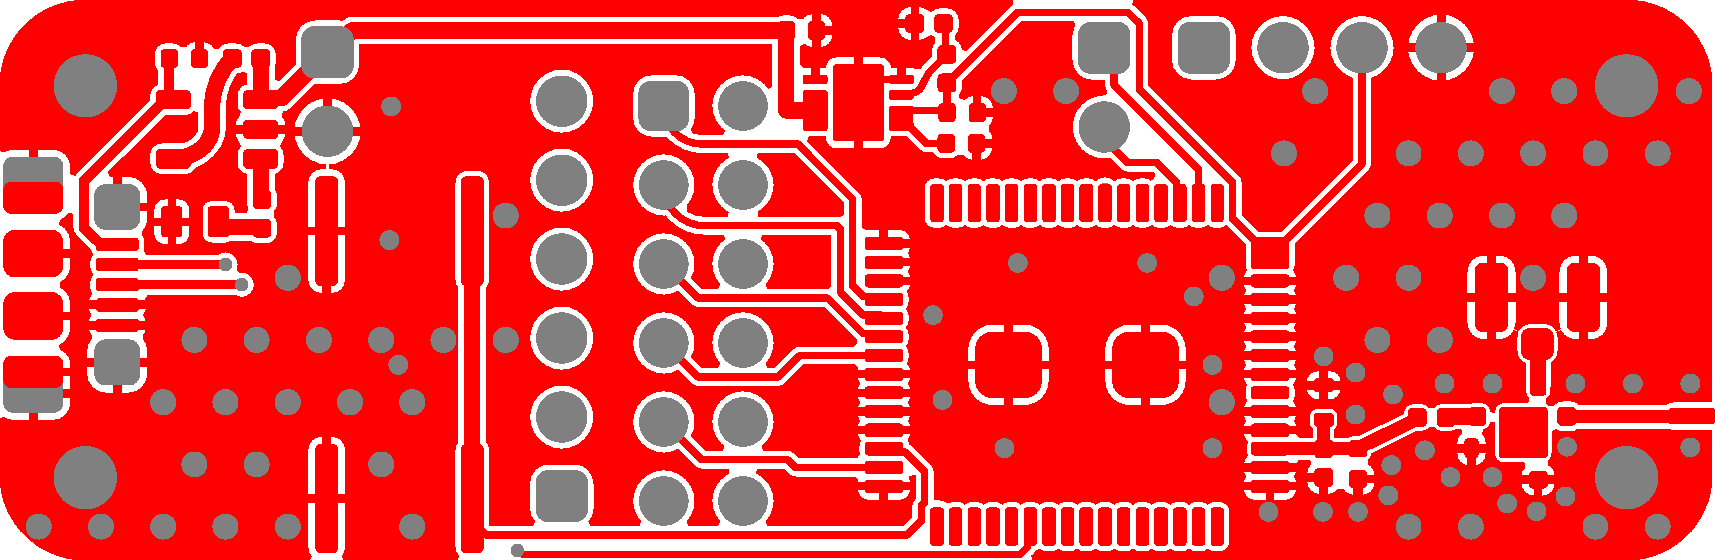
\includegraphics[width=\textwidth, keepaspectratio,angle=50]{MS-Top Layer.pdf}
		\caption{}%
		\label{fig:MS-TopLayer}
	\end{subfigure}
	\hfil
	\begin{subfigure}[c]{0.325\textwidth}
		\centering
		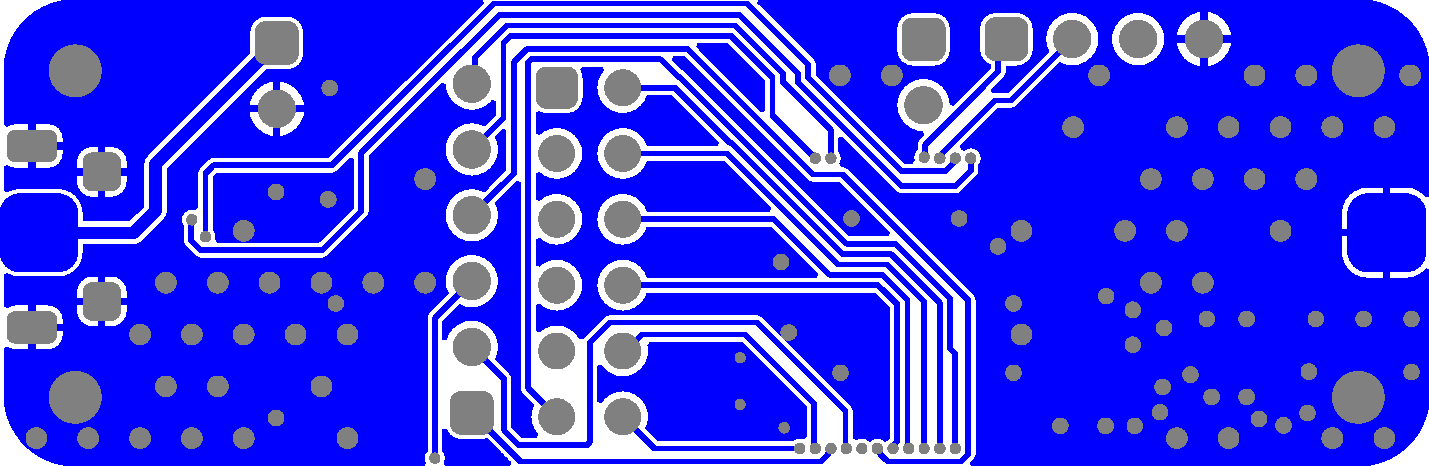
\includegraphics[width=\textwidth, keepaspectratio,angle=50]{MS-Bottom Layer.pdf}
		\caption{}%
		\label{fig:MS-BottomLayer}
	\end{subfigure}
	\hfil
	\begin{subfigure}[c]{0.325\textwidth}
		\centering
		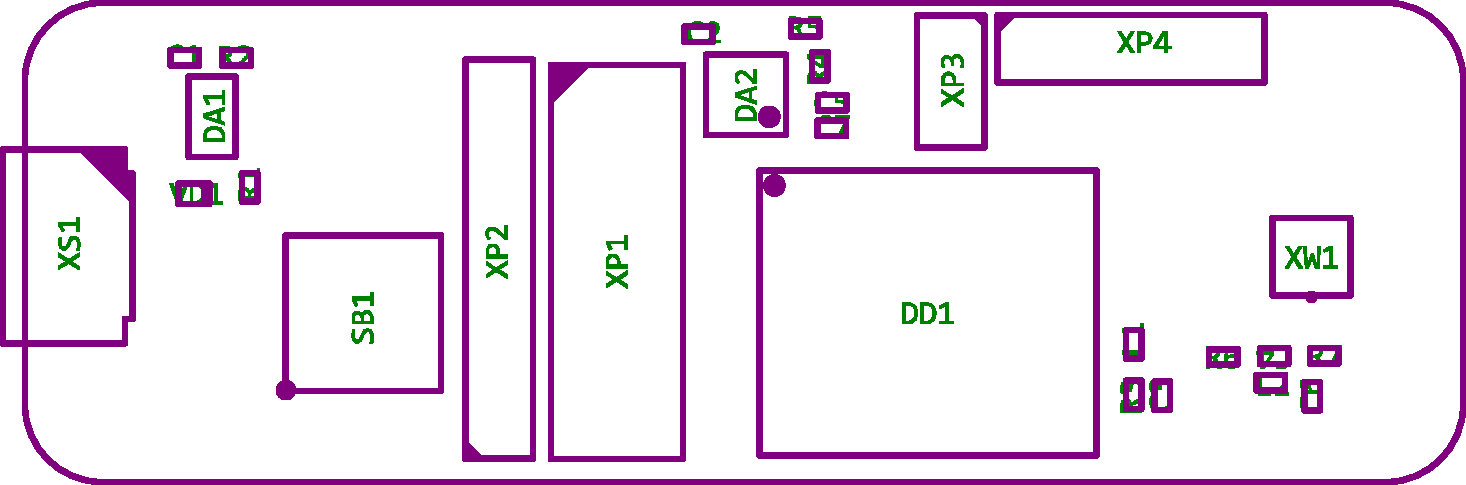
\includegraphics[width=\textwidth, keepaspectratio,angle=50]{MS-Assembly Drawing.pdf}
		\caption{}%
		\label{fig:MS-AssemblyDrawing}
	\end{subfigure}
	\caption{Второй вариант исполнения. Схемы металлизации (а) верхнего и (б) нижнего слоя. (в) сборочный чертёж верхнего слоя.}
	\label{fig:ms-layers}
\end{figure}


\subsection{Трёхмерная модель.}

Для сравнительной оценки размеров и демонстрации итоговых устройств приведём фотореалистичную 3D-модель из инструмента Altium Designer \linebreak Multiboard Assembly View.

\begin{figure}[H]
	\centering
	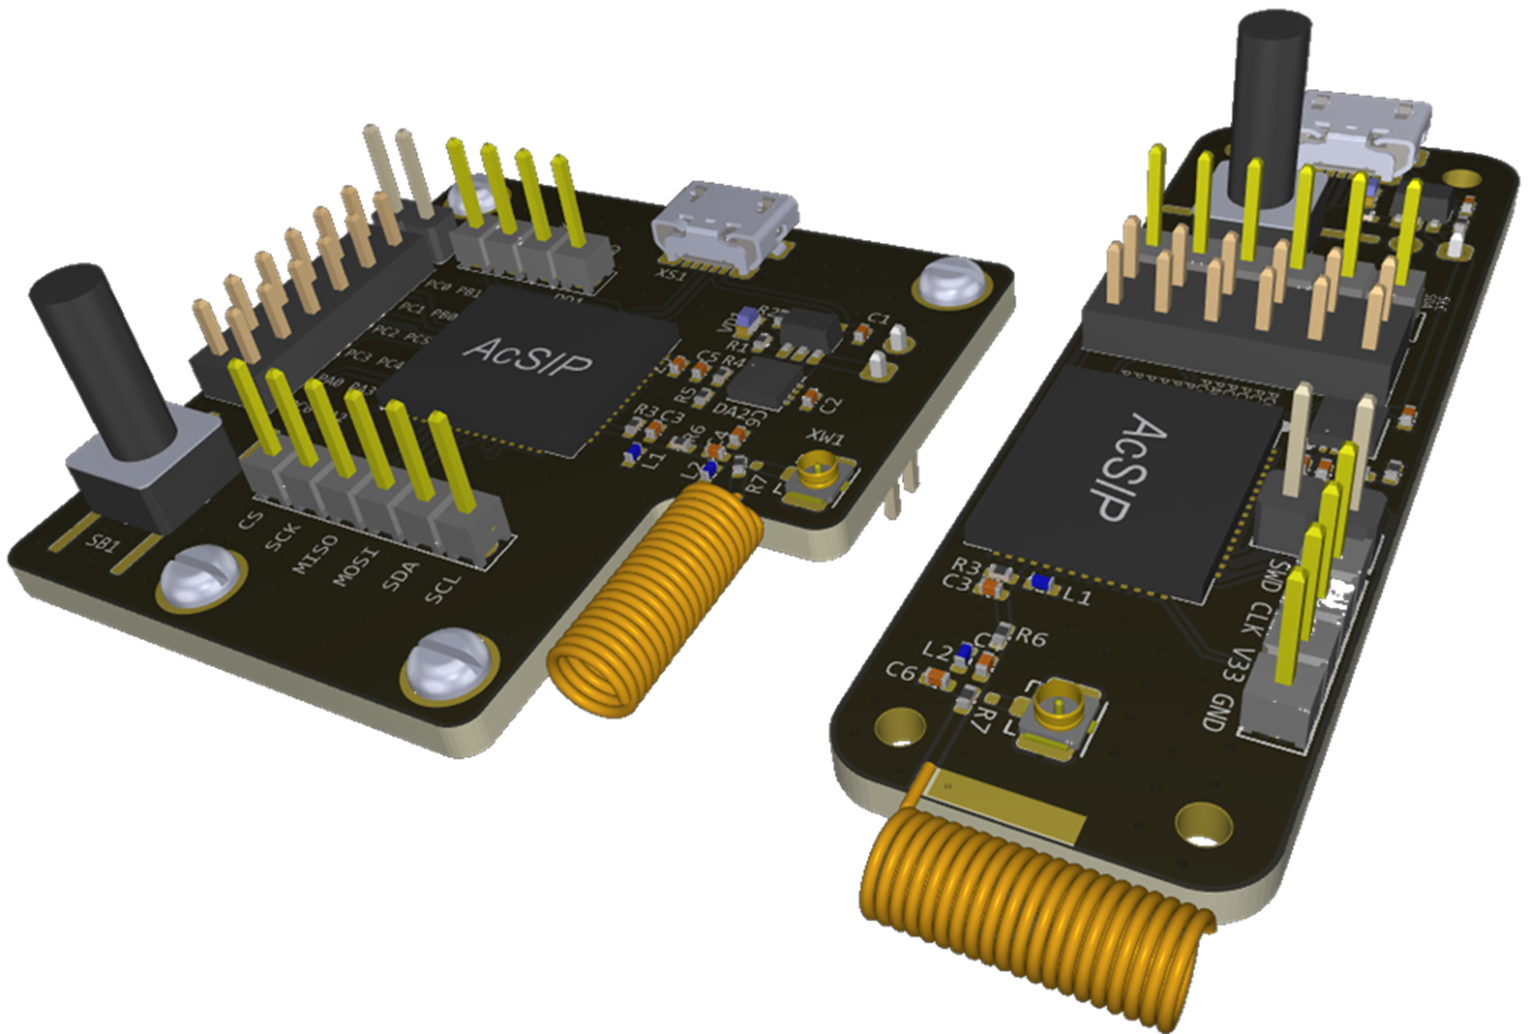
\includegraphics[width=0.7\textwidth,keepaspectratio]{mm-3d-view.png}
	\caption{трехмерные модели плат МОУ, изометрический вид.}
	\label{fig:mm-3d-view}
\end{figure}

